% #############################################################################
% This is Chapter 5
% !TEX root = ../main.tex
% #############################################################################
% Change the Name of the Chapter i the following line
\fancychapter{Forecasting model selection}
\cleardoublepage
% The following line allows to ref this chapter
\label{chap:implementation}

In the past chapters we introduced the theme \ref{chap:intro}, we presented some studies developed in this area \ref{chap:background}, we presented the concrete case studied in this thesis and we proposed a schematization of the work to be developed \ref{chap:architecture}, and we introduced the models that we will implement in this thesis \ref{chap:Model}.
In this chapter, we will present the environment in which the proposed models were trained, the data used and the way how they were treated and used during the research phase, and finally the metrics used to evaluate the performance of the proposed models.
 

\section{Implementation environment} \label{chap5:enviromnet}

During the development of the thesis, several scripts were implemented, both for data processing and for the implementation of machine learning models. The language chosen for this purpose was \textit{Pyhton}. The primary reasons for this choice were the ease of syntax of this language, as well as the large number of libraries available, including \textit{keras}, a Deep Learning library that provides all the necessary tools for building and deploying Neural Networks.

Regarding the hardware components used, two different systems were used during the development of this work. The first environment consists of a CPU (Intel Core i5-3470 3.20GHz), and a GPU (NVIDIA GeForce GTX 1050 Ti) essential to accelerate the training process of the proposed models. The second environment consists of a virtual environment implemented on \textit{Microsoft Azure Machine Learning} platform, where a cluster consisting of a 6 core processor, and a GPU (NVIDIA Tesla K80).

The first environment was used with the purpose of testing, in a first phase, several models with simple tasks, and the second environment was used to put into practice more complex tests that required more computational capacity.
	

\section{Dataset}\label{chap5:dataset}

In this section, we describe the datasets used in the development of this work, and also detail the data preprocessing applied to the datasets so that they had the necessary formatting to be used during this experiment.

\subsection{Data description}

In the day to day of a building, there are many factors that influence its consumption and consequently the available power. In Chapter \ref{chap:background} some examples of work developed with the objective of predicting the energy consumption of a building were mentioned. In Appendix B, Table \ref{table1}, it is possible to verify that generally, two categories of data are used in this kind of applications, data that concern the behavior of the building, and climatic data that characterize the environment in which the building is located.

With respect to data on the behaviour of the building, \ac{EDP} provided two different datasets that present information between January 25, 2020 and September 30, 2020, totalling roughly 8 months of data, with a granularity of 5 seconds. The first dataset includes historical data regarding the energy consumption of the building, and the second dataset includes historical data regarding the solar production generated by the \ac{PV} panels present in the upper part of the building. It is also relevant to mention that the production data provided showed some gaps resulting from sensor reading failures. This aspect implies the need for some mechanisms to complete the missing data.

Regarding climate data, \ac{FCUL} provided two different datasets that present information between January 25, 2020 and June 15, 2020, totaling more or less 5 months of data, with a granularity of 1 minute. The first dataset includes meteorological data regarding the geographical location of the building, and the second includes data regarding solar radiation exerted on the geographical area of the building. Neither of the two datasets had flaws.

In Table \ref{table2}, there is a summary of some key factors regarding the available datasets.


\begin{longtable}{|l|c|c|c|c|}
    \caption{Summary of the datasets used.}
    \label{table2}\\
    
    \hline & \multicolumn{2}{c|}{}&\multicolumn{2}{c|}{}\\[-0.5ex]
    \textbf{Dataset Provider}   & \multicolumn{2}{c|}{\textbf{EDP}} & \multicolumn{2}{c|}{\textbf{FCUL}}\\[1ex]
    \hline & \multicolumn{2}{c|}{}&\multicolumn{2}{c|}{}\\[-0.5ex]

    
    \textbf{Dataset} & \multicolumn{1}{l|}{\textbf{Consumption}} & \textbf{Production} & \multicolumn{1}{l|}{\textbf{Meteorological}} & \textbf{Radiation}  \\
    \textbf{Nº of variables} & \multicolumn{1}{c|}{8} & \multicolumn{1}{c|}{7} &  22  & \multicolumn{1}{c|}{28} \\
    \textbf{Preiod} & \multicolumn{2}{c|}{8 months and 5 days} & \multicolumn{2}{c|}{4 months and 21 days}  \\
    \multicolumn{1}{|r|}{Begin} & \multicolumn{2}{c|}{25-01-2020} & \multicolumn{2}{c|}{25-01-2020} \\
    \multicolumn{1}{|r|}{End}  & \multicolumn{2}{c|}{30-09-2020}  & \multicolumn{2}{c|}{15-06-2020} \\
    \textbf{Nº of days}       & \multicolumn{2}{c|}{249}     & \multicolumn{2}{c|}{142}    \\             
    \textbf{Nº of samples}    & \multicolumn{2}{c|}{4302720} & \multicolumn{2}{c|}{2453760} \\[1ex]
    \hline
    

\end{longtable}

As can be seen through the analysis of Table \ref{table2}, the data provided do not portray the same time window nor have the same granularity. It is then necessary to proceed to some data treatment in order to obtain the data in the desired form.

\subsection{Data manipulation}\label{sec:data_manip}

The data manipulation consists of a process in which the data made available is formatted in such a way that it meets the essential criteria to enable its introduction in the models. During the development of the thesis, this was the most time consuming process. The data treatment is an extremely demanding process, which is simplified in the diagram of Figure \ref{datatreatment}.

\begin{figure}[h!]
    \centering
    \begin{center}
    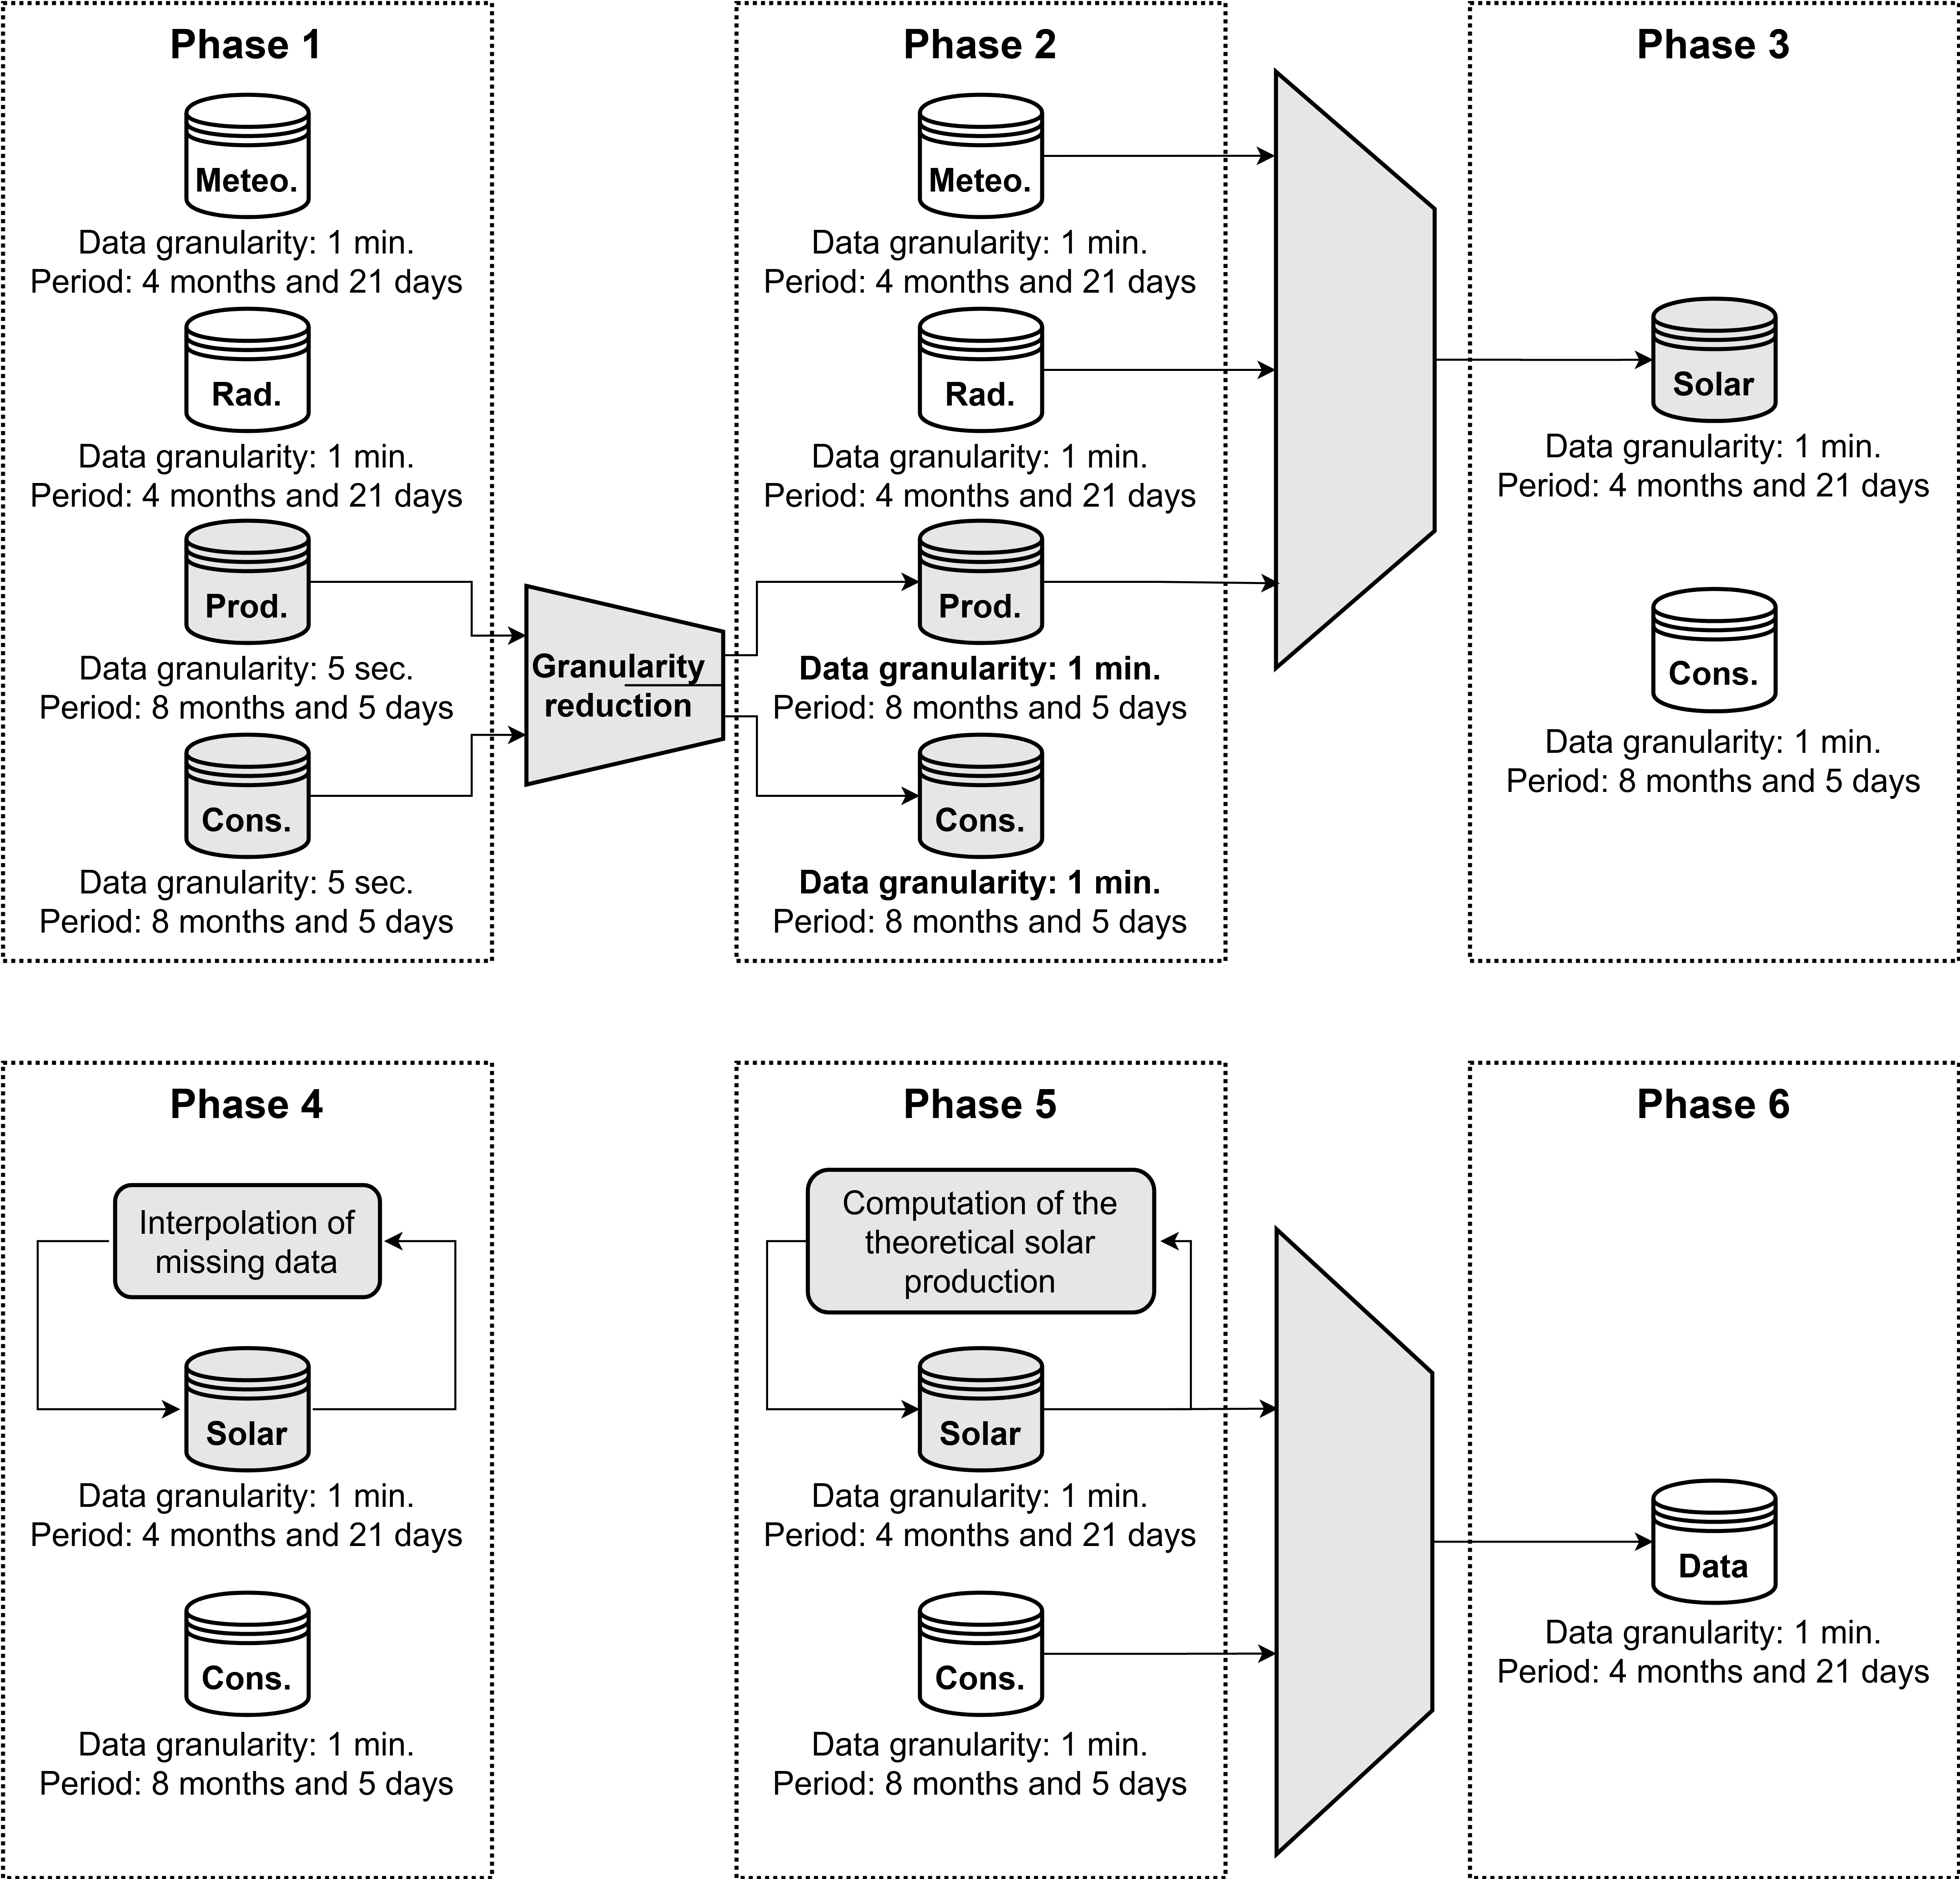
\includegraphics[width=1\textwidth]{Images/Data.png}
    \caption{Data treatment process.}
    \label{datatreatment}
    \end{center}
\end{figure}

In phase 1, the production data (Prod.) is incomplete due to failure of the system responsible for acquiring and storing this indicator. There is also a difference both in granularity and period available, between the data provided by \ac{EDP} and the data provided by \ac{FCUL}. It is then necessary, first of all, to equal the granularity of all four datasets. In order to do that, a function was applied to reduce the granularity of the production (Prod.) and consumption (Cons.) datasets, forcing the frequency of both datasets to one minute. the  The function applies an arithmetic mean given by 

\begin{equation}
     A={\frac {1}{n}}\sum _{i=1}^{n}a_{i}={\frac {a_{1}+a_{2}+\cdots +a_{n}}{n}},
\label{amean}
\end{equation}

where $A$ represents the value of the final measure with frequency of 1 minute, and $n$ represents the number of nodes between that minute range that will be converted to a single value. We then reached phase 2, where the four datasets have the same granularity. Then, the datasets corresponding to the meteorological data (Meteo.), radiation data (Rad.) and production data (Prod.) are concatenated. As a result of this process (phase 3), the dataset (Solar) is formed, which aggregates all the information regarding climate data and solar production data over a period of 4 months and 21 days. The reason behind this phenomenon is that all the production days for which there is no direct correspondence in the meteorological data (Meteo.) and radiation data (Rad.) datasets are rejected. 

As mentioned before, the data regarding the solar production (Prod.) presented some temporal flaws. In order to solve the problem, two solutions were found. For time gaps of less than 30 minutes (phase 4), a quadratic interpolation was applied. As an example, given any three points $(x_0, f(x_0))$, $(x_1, f(x_1))$ and $(x_2, f(x_2))$, the polynomial that interpolates the three points is given by

\begin{equation}
\begin{split}
     & f_2(x)=b_0+b1(x-x_0)+b_2(x-x_0)(x-x1),\\
     & where:\\
     & b_0=f(x_0),\\
     & b_1=f[x_0,x_1]=\frac{f(x_1)-f(x_0)}{x_1-x_0},\\
     & b_2=f[x_0,x_1,x_2]=\frac{\frac{f(x_2)-f(x_1)}{x_2-x_1}-\frac{f(x_1)-f(x_0)}{x_1-x_0}}{x_2-x_0}.\\
\end{split}
\label{poly}
\end{equation}

In order to exemplify the evolution of the incomplete dataset construction, in the graph of Figure \ref{int0} we can observe the solar power generated measured by the sensors on February 3, 2020. In red, is the portion of data that were measured, corresponding to the Solar dataset in Phase 3 represented in Figure \ref{datatreatment}. After the interpolation, to the original dataset are added the points represented in blue, which represent measurement failures of less than 30 minutes. At the end of Phase 4, the dataset is then composed of the data points represented in blue plus the points represented in red.



\begin{figure}[h!]
    \centering
    \begin{center}
    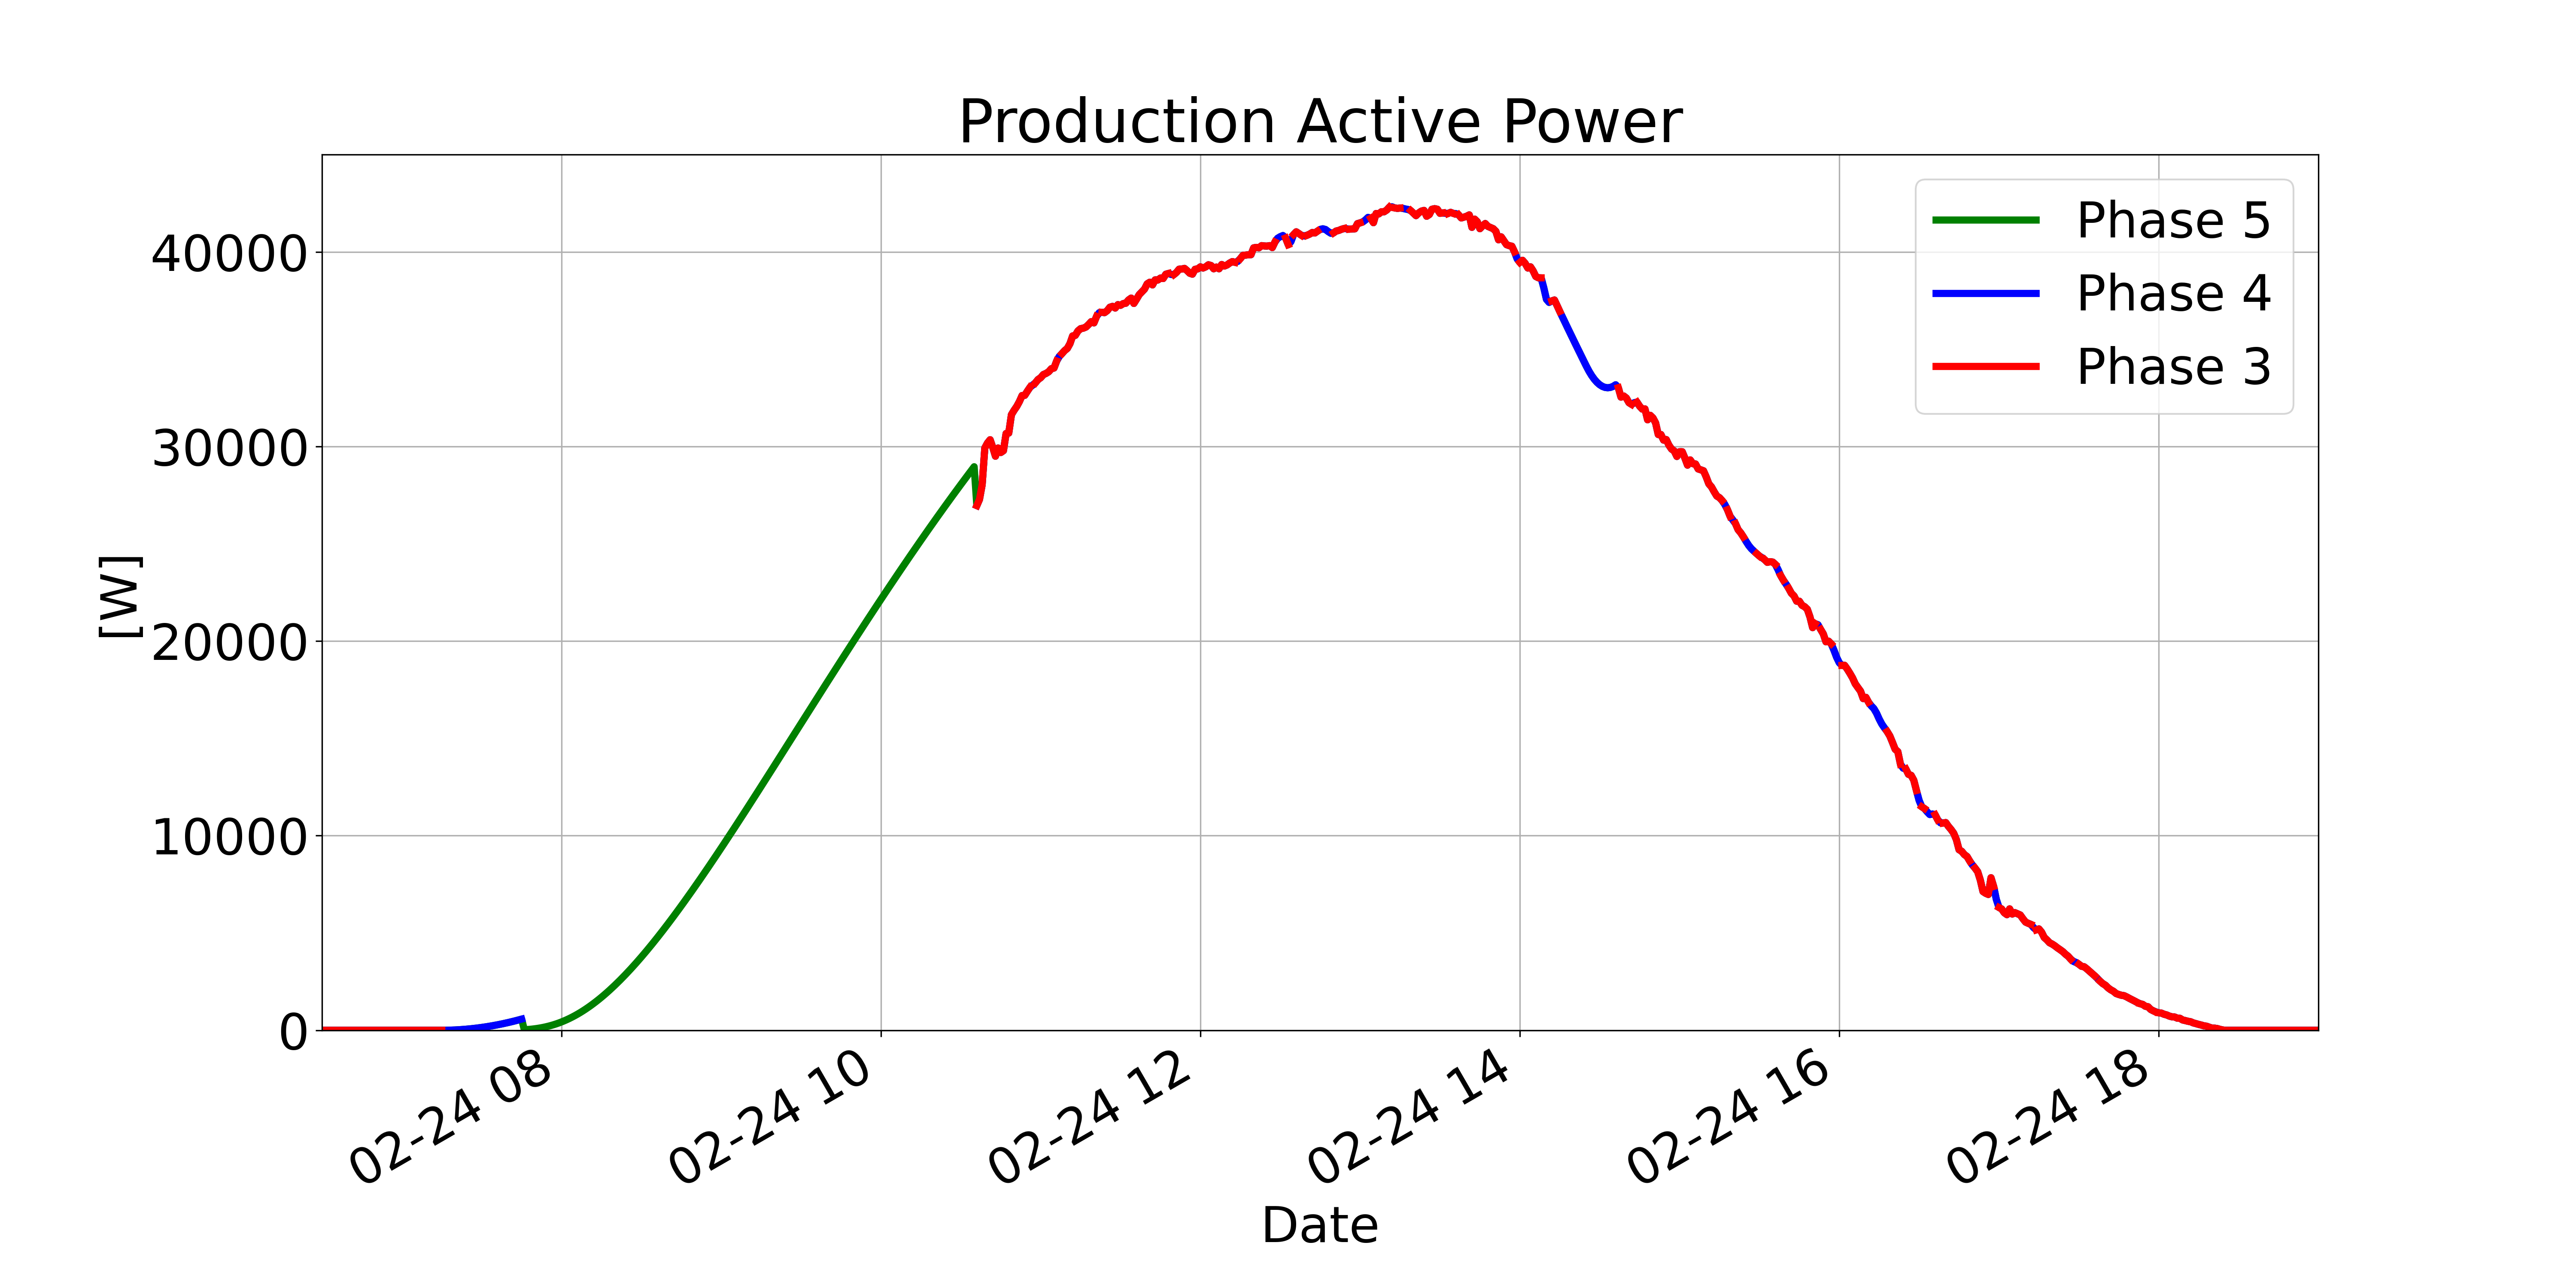
\includegraphics[width=1\textwidth]{Images/int0.png}
    \caption{Data treatment process.}
    \label{int0}
    \end{center}
\end{figure}





For time failures of more than 30 minutes, the dataset was completed with theoretically computed values, since the interpolation for large temporal failures does not present the expected behavior.
Based on the equation of the sun's position in the sky throughout the year, the maximum amount of solar insolation on a surface at a particular tilt angle can be calculated as a function of latitude and day of the year\cite{solar0}. In order to determine the direct component of solar radiation in $kW/m^2$, we used


\begin{equation}
     I_D = I_0*0.7^{(AM^{0.678})}
\label{solar}
\end{equation}

where $I_0$ is the solar intensity external to the Earth's atmosphere that is approximately $1.353 kW/m^2$, $0.7$ represents the overall attenuation of the atmosphere, $AM = \frac{1}{cos\theta}$ is the airmass and $\theta$ is the zenith angle (90° minus the altitude) of the sun. This formula produces an optimal result when there are no clouds. Multiplying the resulting value by the total area of panels in the building and taking into account their positioning efficiency, a theoretical value of power generated by the \ac{PV} panels is obtained, in an ideal scenario. In Phase 5, all missing readings were replaced by the calculated theoretical value, as can be seen in Figure \ref{int0} in green. This way, the Solar dataset was completed. It is possible to verify that the point of change between the theoretical data (the green one) and the original data (the red one) is somewhat sudden, because the green signal considers an ideal scenario and the red signal represents real measurements (affected by clouds, cranes, etc.) The sum of the green, blue and red signals, result in a complete signal for the solar active power generated by the \ac{PV} panels.


In Phase 6 the Solar and Cons. datasets were concatenated, thus reducing the dataset time interval to a final result of 4 months and 21 days.



\subsection{Feature selection}

Although a huge amount of data was made available for the development of this study, the use of a large number of different features may negatively affect the performance of the tested models, namely their speed. In order not to overload the models, an initial set of features from all the available datasets was selected. In Table \ref{table3} the reader may find the selected features, their unit and their descrption.


\begin{longtable}{|l|c|l|}
    \caption{Features used.}
    \label{table3}\\
    
    \hline 
    & &\\[-0.5ex]
    \textbf{Feature}   & \textbf{Unit} & \textbf{Description}\\[1ex]
    \hline
     & &\\[-0.5ex]
    \textbf{$Std\_DHI$} & $W/m^2$ & Standard diffuse horizontal irradiance\\
    \textbf{$Avg\_DHI$} & $W/m^2$ & Average diffuse horizontal irradiance \\
    \textbf{$Avg\_GHI$} & $W/m^2$ & Global horizontal irradiance \\
    \textbf{$Avg\_DNI$} & $W/m^2$ & Direct normal irradiance \\
    \textbf{$Avg\_POA$} & $W/m^2$ & Average plane of array\\
    \textbf{$T\_amb\_avg$} & $^\circ C$ & Average ambient temperature\\
    \textbf{$Theoretical Value$} & $W$ & Theoretical production active power generated\\
    \textbf{$ActPwr$} & $W$ & Production active power\\
    \textbf{$Ir$} & $A$ & Consumption three-phase current \\
    \textbf{$Is$} & $A$ & Consumption three-phase current \\
    \textbf{$It$} & $A$ & Consumption three-phase current \\
    \textbf{$Vrs$} & $V$ & Consumption three-phase voltage\\
    \textbf{$Vst$} & $V$ & Consumption three-phase voltage\\
    \textbf{$Vtr$} & $V$ & Consumption three-phase voltage\\
    \textbf{$P$} & $W$ & Consumption real power\\
    \textbf{$S$} & $VA$ & Consumption complex power\\
    \textbf{$hour$} & $hours$ & Hour of the day\\
    \textbf{$day\_of\_month$} & $days$ & Day of the month\\
    \textbf{$day\_of\_week$} & $days$ & Day of the week\\
    \textbf{$month$} & $months$ & Month of the year\\
    \textbf{$holiday$} & $binary$ & National holiday identifier\\[+1ex]
    \hline
    

\end{longtable}

Although all these features contribute in some way to enrich the past information available, it is important to reduce as much as possible the number of features used as input to the model, limiting the choice to the essentials.
In this sense, a second phase of analysis was then carried out where the correlation matrix between each of the features was projected. In Figure \ref{corr} one can then observe the correlation matrix where the correlations between all the selected variables are represented. The value of the correlation is present in the [-1, 1] range, where -1 means that the variables present an opposite correlation, 0 means that there is no correlation between the two variables and 1 means that there is perfect correlation between the two variables. 


\begin{figure}[h!]
    \centering
    \begin{center}
    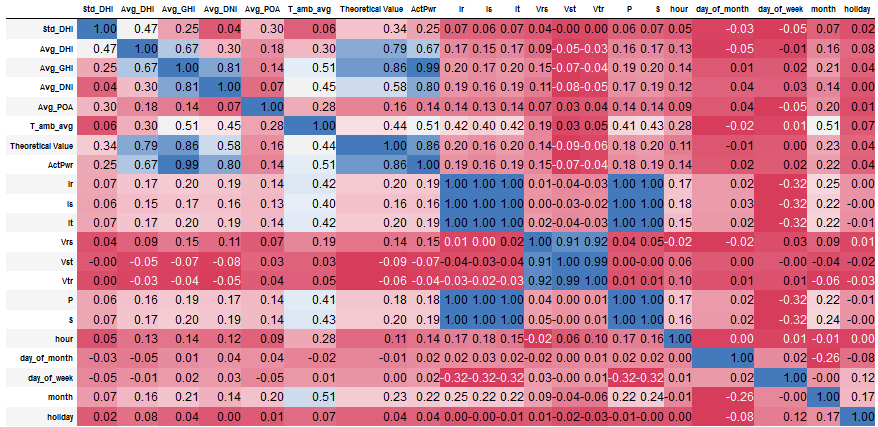
\includegraphics[width=1\textwidth]{Images/corr.PNG}
    \caption{Feature correlation matrix.}
    \label{corr}
    \end{center}
\end{figure}


The aim of computing this matrix is to identify variables that present a perfect or almost perfect correlation between them, in order to eliminate redundancies. 

A perfect correlation between two variables means that one can be deduced from the other, that is, the relevance of the two variables for the construction of the forecasting system is the same, so one of the variables can be eliminated. 


First of all, it was decided to eliminate the features that contribute to the calculation of others. In this sense, both three-phase voltages and three-phase currents contribute to the calculation of $S$ and $P$ and present a perfect correlation between them. It was then chosen to eliminate the features: $Ir$, $Is$, $It$, $Vrs$, $Vst$, $Vtr$. Then, since in this case $S$ does not have an imaginary component, $S$ and $P$ have the same value. The feature $S$ was then also eliminated. Also, although $Theoretical\ Value$ and $Avg\_GHI$ present a very high correlation with $ActPwr$ (which is predictable given that the measured $ActPwr$ these two variables were added, as explained in section X), we chose to keep these two variables as input features since the correlation is not exactly perfect and can be decisive in certain cases in building a good predictive model. Therefore, the variables chosen for the input of all tested models are: $Std\_DHI$, $Avg\_DHI$, $Avg\_GHI$, $Avg\_DNI$, $Avg\_POA$, $T\_amb\_avg$, $Theoretical\ Value$, $ActPwr$, $P$, $hour$, $day\_of\_month$, $day\_of\_week$, $month$ and $holiday$. In addition, the variable $Available Powe$ given in $watts$ has been added as an input feature, resulting in a total of 15 input features and 1 output.



SLIDING WINDOWXXXXXX

\subsection{Data partition}\label{sec:datap}

In order to study a certain algorithm, it is necessary to have access to past data to train the model and then evaluate its performance. The the available data as well is an important factor when it comes to developing predictive models. Usually, in \ac{ML}, to study a certain model, the dataset should be divided into three sets as can bee seen in Figure \ref{division}. 

\begin{figure}[h!]
    \centering
    \begin{center}
    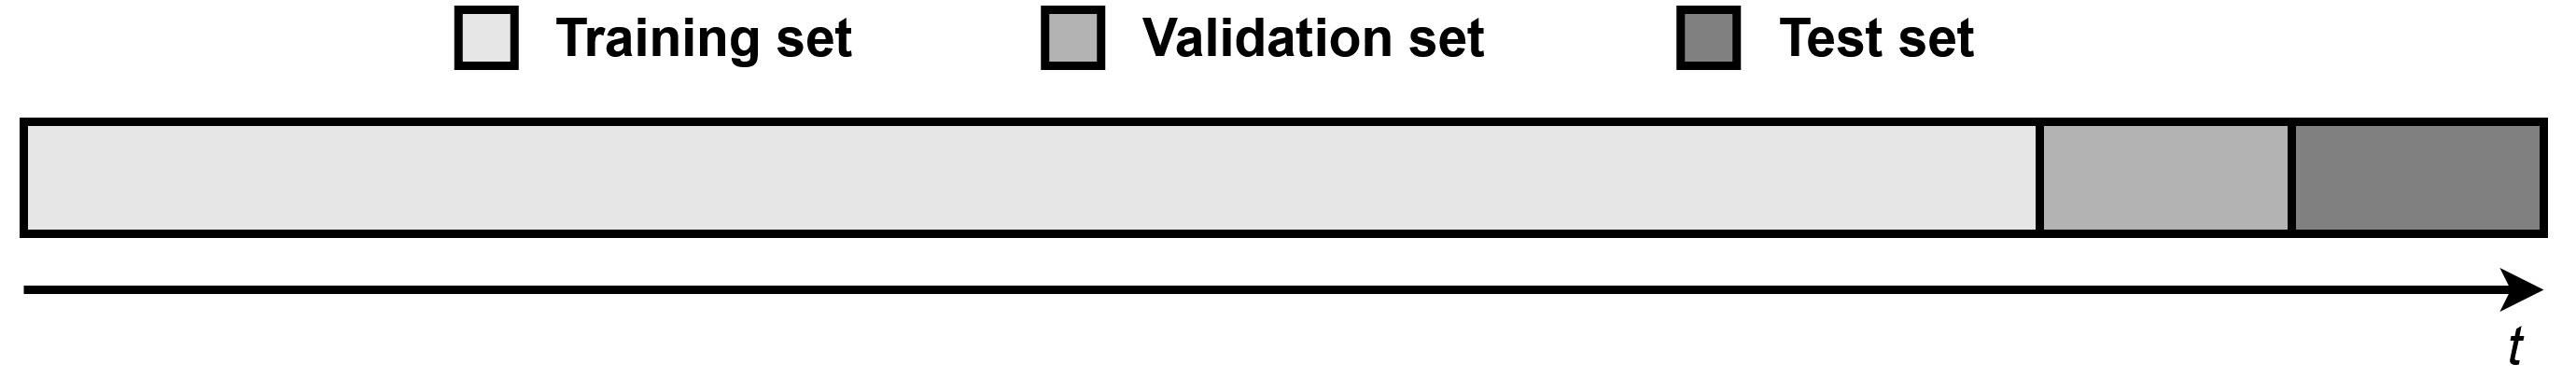
\includegraphics[width=1\textwidth]{Images/division.png}
    \caption{Dataset division.}
    \label{division}
    \end{center}
\end{figure}

The first set is known as a training set, and consists of a dataset used to feed the model with examples in order to fit the hyperparameters, such as the weights of connections between neurons in artificial neural networks. As the name implies, the training set is suitable to train the model, progressively adapting the model to its intended purpose. The second is the validation set, which is responsible for simultaneously continuing to adapt the hyperparameters of the model, while providing an unbiased evaluation of the model fit. In addition to that, it can be used for regularization, as is the case of eraly-stopping, referred to in section \ref{sec:early}. Finally, the test set is an independent dataset of the two previous ones, which has as main objective to evaluate in an unbiased way the performance of the model in unseen data (data that was not used neither in the training process nor in the validation process). 

In this study, a distribution with 80\% of training data, 10\% of validation data and 10\% of test data was used. Other combinations were tested as 90\% - 5\% - 5\% and 70\% - 15\% - 15\%, but always obtained poorer results. 

One way to use the available dataset to evaluate the proposed models would be to simply apply the standard training-validation-testing division to the entire dataset available, but this strategy would be a poor way to use the small amount of data available. Typically, to evaluate machine learning models on a very limited time interval, k-fold cross-validation is used. However, cross-validation can present some problems when applied to time-series problems, since one cannot choose random samples and assign them to either the test set or the training set because it makes no sense to use future values to predict past values. There is a time dependency between observations, and it is essential to preserve this relationship during testing. To overcome this barrier, a block cross-validation method was used.

In Figure \ref{partition} the reader may find four different sub-datasets, resulting from a division of the main datastet, defined in phase 6, of the section \ref{sec:data_manip}. The idea behind this division is, in a first part, to use datasets 1, 2 and 3 for training and validation in order to make hyperparameter tuning, and use dataset 4 to test the final models.

\begin{figure}[h!]
    \centering
    \begin{center}
    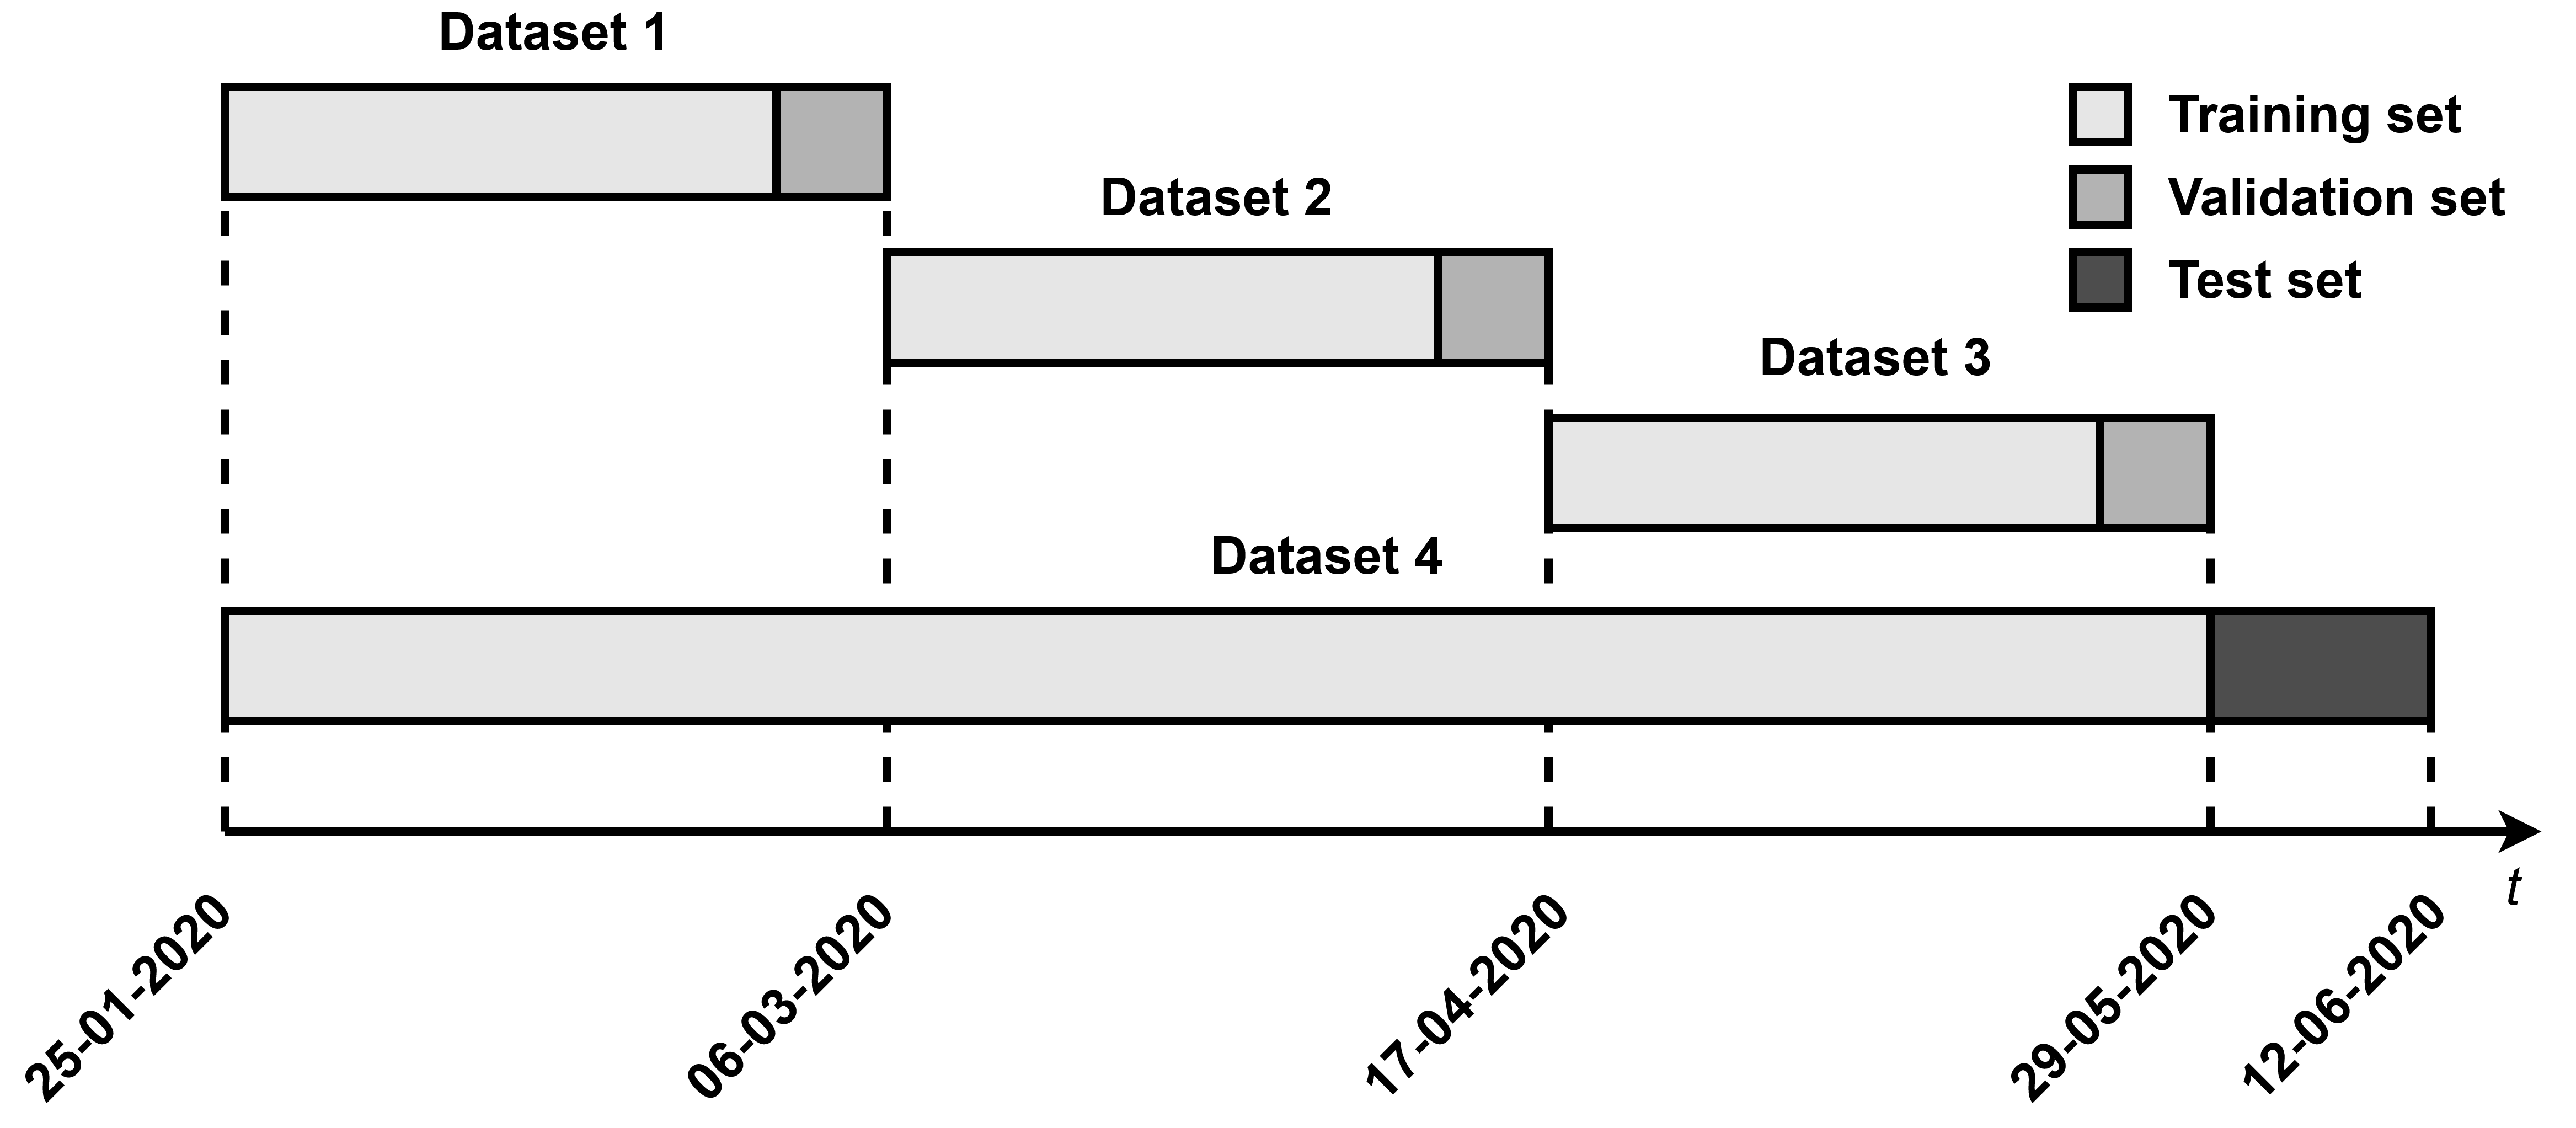
\includegraphics[width=1\textwidth]{Images/data_partition.png}
    \caption{Data partition diagram.}
    \label{partition}
    \end{center}
\end{figure}

Datesets 1, 2 and 3 feature five weeks of training and one week of validation. The dataset 4, however, presents 18 weeks of training and two tests. The overall goal is to propose a model capable of predicting the available power between May 25 and June 12. The standard approach would be to split dataset 4 in training, validation and testing.  Block cross-validation consists of dividing the training set in a fixed number of blocks, and perform training and validation on these blocks. The overall performance evaluation of the models is then given by the average of the performance in each of these blocks i.e., the error of the models is given by

\begin{equation}
     Model\ error =\frac {1}{k}\ \sum_{i=1}^k Error_{di},
\label{err_av}
\end{equation}

where $Model\ error$ represents the final model error, and $Error_{di}$ represents the error that the model presented while performing in dataset $i$, and $k$ represents the number of datasets used.
In this specific case, the validation error for each model is given by

\begin{equation}
     Model\ error =\frac {1}{3}\ (Error_{d1} + Error_{d2} + Error_{d3}).
\label{err_av}
\end{equation}

The great advantage of using this method is the reduction of the influence of eventual points in the choice of the best model. In other words, by performing an average of 3 different sets, the robustness of the choice process is increased since different scenarios are considered and the best model is the one that performs well on average for all of them.

\section{Performance evaluation metrics}\label{chap5:evaluation}

In the previous section, important details concerning the data used in this thesis were explained. One defined $Model\ error$, but did not specify which concrete metrics were used in this work. To compare the performance of the different models in the defined dataset, it is necessary to use some measures of forecast performance. In this sense, during this thesis four different measures were used that relate the real values present in the time series represented by $y_t$, and the forecast values, which are represented by $f_t$. Thus, the forecast error is given by $e_t=y_t-f_t$. The three measures presented are quite common in the literature \cite{} and are described below.

\subsection{Mean Absolute Error (MAE)}

The \ac{MAE}, is defined as

\begin{equation}
     MAE =\frac {\sum_{t=1}^n|e_t|}{n}.
\label{mae}
\end{equation}

The \ac{MAE} is known as a scale-dependent accuracy measure and measures the average absolute deviation between the forecasted values and the real ones. As a scale-dependent measure, it cannot be used to compare series series using different scales.


\subsection{Mean Squared Error (MSE)}

The \ac{MSE}, is defined as

\begin{equation}
     MSE =\frac {1}{n}\sum_{t=1}^ne_t^2.
\label{mse}
\end{equation}

The \ac{MSE} is also known as a scale-dependent accuracy measure and measures the average squared deviation between the forecasted values and the real ones. The application of this measure is quite relevant because it doesn't allow the negative errors to cancel the positive errors and vice-versa. 

\subsection{Root Mean Squared Error (RMSE)}

By applying the square root to the \ac{MSE}, the \ac{RMSE} is then defined as

\begin{equation}
     RMSE =\sqrt{MSE} = \sqrt{\frac {1}{n}\sum_{t=1}^ne_t^2}.
\label{rmse}
\end{equation}

The advantage of \ac{RMSE} over \ac{MSE} is that it is on the same scale as the targets, facilitating its interpretation in the concrete context of the problem. 

\section{Algorithm selection} \label{chap5:framework}

In this section, we explain the 8 architectures introduced in the section \ref{sec:arq}, and describe the method used to optimize the hyperparameters of each of the models. In addition, we also choose the models that present the best performance for specific situations such as holidays and weekends. At the end of this section, the goal is to find a model or a set of models that present good overall performance.


\subsection{Part 1 - Hyperparameter tuning}\label{sec:part1}
In the first part of the process, the focus was to optimize the hypterparameters of the 8 proposed architectures in order to obtain the best set of hyperparameters for each of the eight architectures. To do so, a script was developed responsible for training and validating all possible combinations of different hyperparameters (within a predefined range), for each one of the 3 Datasets mentioned in section \ref{sec:datap}. In Table \ref{table4} the different combinations of hyperparameters tested for each of the architectures can be observed.

\begin{longtable}{|c|c|c|c|}
    \caption{Combinations of hyperparameters tested.}
    \label{table4}\\
    \hline 
    & & & \\[-0.5ex]
    \textbf{Model} & \textbf{Architecture}   & \textbf{Hyperparameters tested values} & \makecell*[{{p{2.5cm}}}]{\centering\textbf{Total number of combinations}}\\[3ex]
    \hline
    & & & \\[-2ex]
    Model 0 & GRU & \makecell*[{{p{6.3cm}}}]{\centering Units - [8, 16, 32, 64, 128, 256, 512]} & 7\\
    \hline
    Model 1 & LSTM & \makecell*[{{p{6.3cm}}}]{\centering Units - [8, 16, 32, 64, 128, 256, 512]} & 7\\
    \hline
    Model 2 & 1D CNN - GRU & \makecell*[{{p{6.3cm}}}]{\centering Filters - [8, 16, 32, 64, 128, 256], Kernel\_size - [10,60], \\Units - [8, 16, 32, 64, 128, 256]} & 72\\
    \hline
    Model 3 & 1D CNN - LSTM & \makecell*[{{p{6.3cm}}}]{\centering Filters - [8, 16, 32, 64, 128, 256], Kernel\_size - [10,60], \\Units - [8, 16, 32, 64, 128, 256]} & 72\\
    \hline
    Model 4 & GRU - GRU & \makecell*[{{p{6.3cm}}}]{\centering Units - [8, 16, 32, 64, 128] (2x)} & 25\\
    \hline
    Model 5 & LSTM - LSTM & \makecell*[{{p{6.3cm}}}]{\centering Units - [8, 16, 32, 64, 128] (2x)} & 25\\
    \hline
    Model 6 & GRU - LSTM & \makecell*[{{p{6.3cm}}}]{\centering Units - [8, 16, 32, 64, 128] (2x)} & 25\\
    \hline
    Model 7 & LSTM - GRU & \makecell*[{{p{6.3cm}}}]{\centering Units - [8, 16, 32, 64, 128] (2x)} & 25\\
    \hline
    & & & \\[-0.5ex]
    \textbf{Total} & \textbf{-} &  \textbf{-} & \textbf{258}\\[+1ex]
    \hline
    

\end{longtable}

Models 0, 1, 4, 5, 6 and 7 only consist of \ac{GRU} and/or \ac{LSTM} layers. In this type of layers, the hyperparameter that changed was only the number of Units - A positive integer that represents the dimensionality of the output space. In models 4, 5, 6 and 7, these values are combined 2 to 2 (8-8, 8-16,... 128-64, 128-128), producing 25 different combinations. On Models 2 and 3, the parameters that are varied are the number of filters of the \ac{1D CNN} - An integer that represents dimensionality of the output space (i.e. the number of output filters in the convolution), the kernel\_size of the \ac{1D CNN} - An integer or tuple/list of a single integer, specifying the length of the 1D convolution window used, and again, the number of Units of the \ac{GRU} and \ac{LSTM} layers. With all these variants, 258 different models are then built and put to the test. The function of this first step is to reduce these 258 models to the best 8, thus selecting the best hyperparameters for each of the 8 architectures. It should be mentioned that, although after the treatment carried out in Part 1 the ideal hyperparameters for each of the 8 network structures are obtained, these values should only be used as indicators. If one verifies that the change of a parameter affects positively the model, then this change should be made.


In Appendix C, Table \ref{table7}, 













\subsection{Part 2 - Situational study}

In the second part of the process, the main objective is to compare the 8 models chosen in Part 1, situationally. To bring this into practice, multiple subdasets were created presenting particular situations in the activity of the building such as weekends, holidays, etc.

This step serves to identify which model presents the best performance depending on the situation to be expected. If it is possible to define a model that is clearly better to predict certain situations, and another that presents better performance in others, there is the possibility of creating a superior abstraction layer capable of choosing the best model to use in a given scenario. In Table {} are present the different scenarios tested as well as the number of cases used in choosing the best model for the scenario in question.

\begin{longtable}{|c|c|}
    \caption{Scenarios tested.}
    \label{table5}\\
    \hline 
    & \\[-0.5ex]
    \textbf{Scenario} & {\centering\textbf{Total number of cases}}\\[1ex]
    \hline
    & \\[-0.5ex]
    National holiday & 6\\
    Weekends & X\\
    Rainy days & \\
    Cold days & \\[1ex]
    \hline
    

\end{longtable}

For each of the cases presented in Table \ref{table5}, a dataset was created whose training subset represents the scenario to be tested. In order to understand which of the 8 models presents the best performance for each scenario, the equation \ref{err_av} was used again. Applying a specific case, the best model to apply in a holiday scenario will be the one that presents on average the lowest error value in the 6 scenarios where it was tested.

\subsection{Part 3}

\subsection{Framework diagram}


\section{Conclusion}

In this chapter, we have delved into the whole process of implementing the work of this thesis. Initially, in the section \ref{chap5:enviromnet}, we describe the different implementation environments used, and then, in the section \ref{chap5:dataset}, we describe the datset used and all the data processing that was performed. In the section \ref{chap5:framework}, we present the test framework and the process chosen to select the best models. Finally, in the section \ref{chap5:evaluation}, we describe the metrics used to choose the best models designed.